% CAPT
%
% !TEX root = ../thesis-main.tex
%

\chapter{Computer-Assisted Pronunciation Tutoring}

%\cleanchapterquote{You can’t do better design with a computer, but you can speed up your work enormously.}{Wim Crouwel}{(Graphic designer and typographer)}

\blindtext 
\section{Pronunciation in foreign language teaching}
\blindtext
\section{CAPT systems}
	\subsection{Selecting errors to target}
	\blindtext
		\begin{center}
		\begin{figure}[htb]
			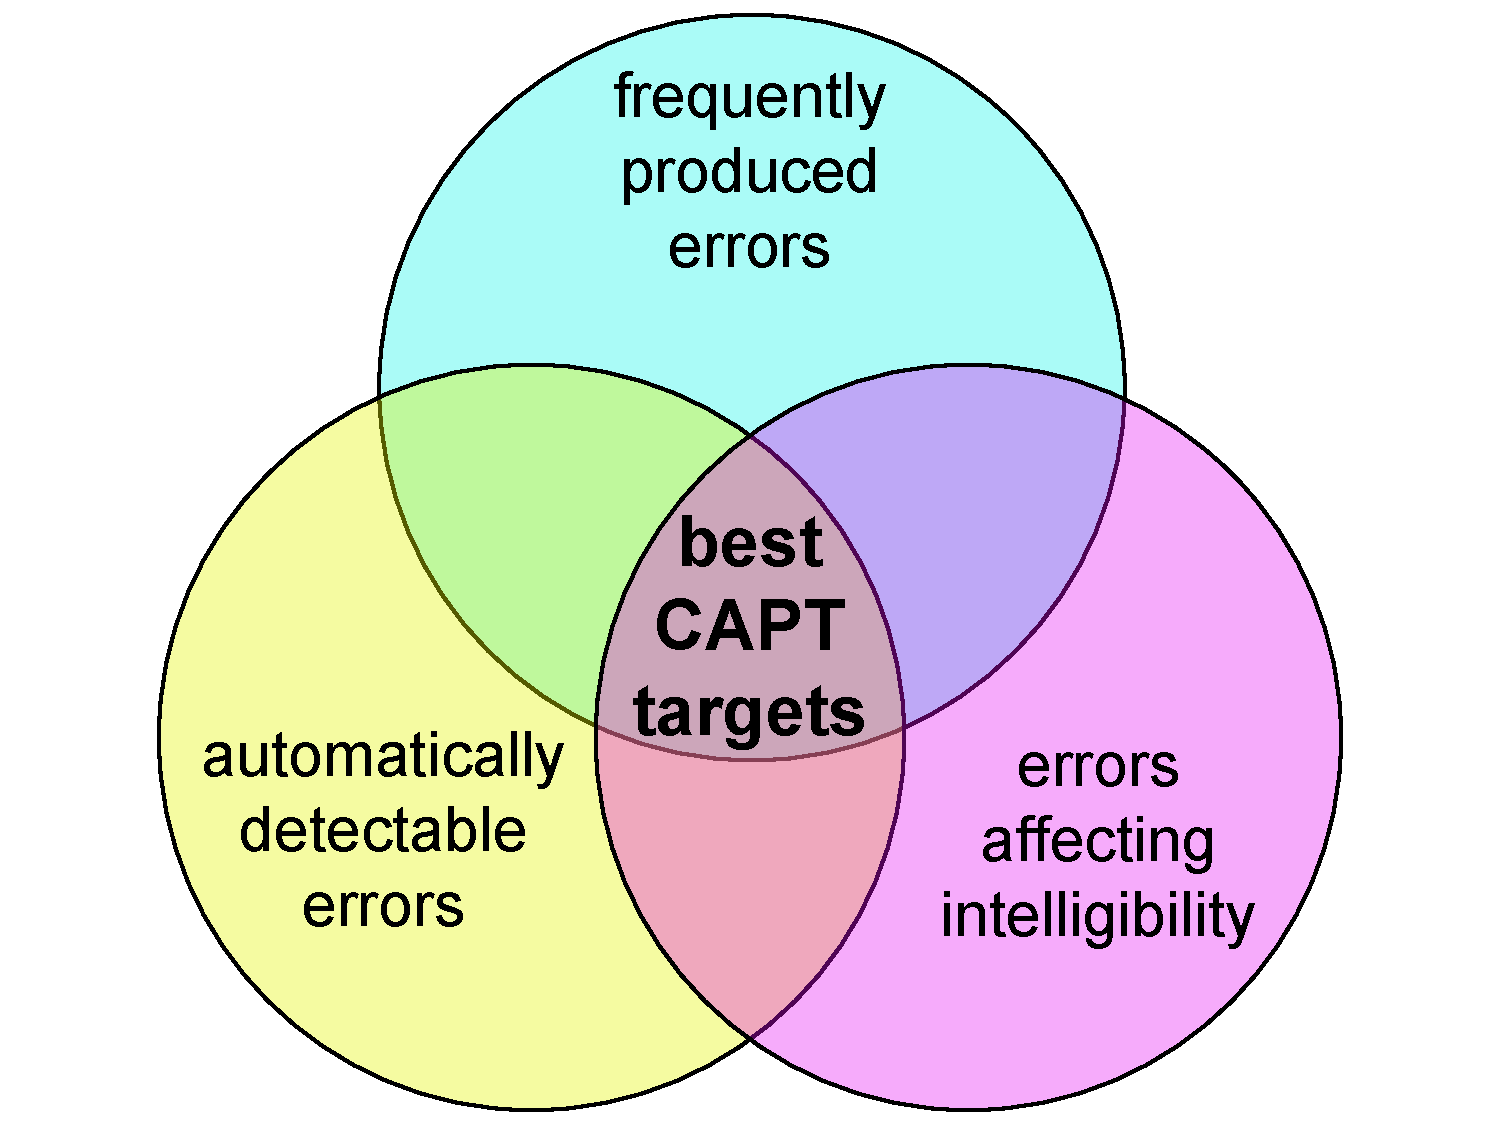
\includegraphics[width=.7\textwidth]{../img/error-venn}
			\caption{Criteria for selecting errors to target in a CAPT system.}
			\label{fig:errors}
		\end{figure}
		\end{center}
	\subsection{Survey of existing CAPT systems}
	
\section{The IFCASL project}
	\subsection{Individualized feedback in CAPT?}
	\subsection{The IFCASL corpus}

